\chapter{Experimental Evaluation}\label{chapter:experiments}
In this section we describe the experimental environment and provide details about the criteria we chose to focus on, and the steps followed in our experiments. Besides that, we discuss the corresponding results. The project's source code and other supplementary material are available on GitHub\footnote{\url{https://github.com/perikost/ExploringEthereum}}.

Before proceeding further, we should mention an important detail concerning the data we used during our experiments. Solidity uses UTF8 encoding, according to which common ASCII characters are represented by a single byte. Additionally, generating random fixed-length character sequences is simple and all the methods we examined support this format. So, to evaluate the cost of storage in Ethereum, for each test case, we recorded 15 measurements regarding various string sizes equally spread across the range of 1B-16KB. However, for those cases that exhibited consistent behavior we present only part of our measurements.

\section{Experimental Setup}\label{sec:}
\subsection{Local experiments}\label{sec:}
We conducted our experiments on a machine with i7-8700 CPU, 64GB RAM, 2TB SSD running Ubuntu 20.04. All SCs were written and compiled in Solidity 0.8.12 with the optimizer disabled and were deployed on Ropsten Testnet. Geth version 1.10.16 was used as an Ethereum client. For IPFS and Swarm, IPFS-client version 0.7.0 and Swarm Bee Client version 0.5.0 were used, respectively.
\subsection{Remote Experiments}\label{sec:}
Grid5000...
\section{Criteria}\label{sec:}
For evaluating the sustainability of using Ethereum as a stand-alone data store, we emphasized on the associated gas cost. In this regard, we thoroughly examined the \hl{most common storage methods}, the SC storage, and the event-logs. Considering these as reference points, we explored alternatives and cost-wise compared the resulting gas costs. In addition, the implementation complexity of each approach was considered. Our findings are summarized in Table~\ref{table:overall}. \hl{On the other hand, the respective costs of the hybrid schemes are presented} in Table~\ref{tab:hash_cost}. Among others, the results confirm that the use of SC storage incurs costs that are orders of magnitude larger than the alternative data stores we examined.

Except for being monetarily viable, DApps need to perform adequately when it comes to retrieving data. That being said, we measured the retrieval time in all the above scenarios. \hl{For IPFS and Swarm, both upload and retrieval performances were taken into account, aiming to a better overall comparison.}
\section{Storing Data in Ethereum}\label{sec:evaluation_ethereum}
\subsection{SC Storage}\label{subsection:evaluation_sc}
\begin{figure}[htbp]
    \begin{subfigure}{\linewidth}
        \centerline{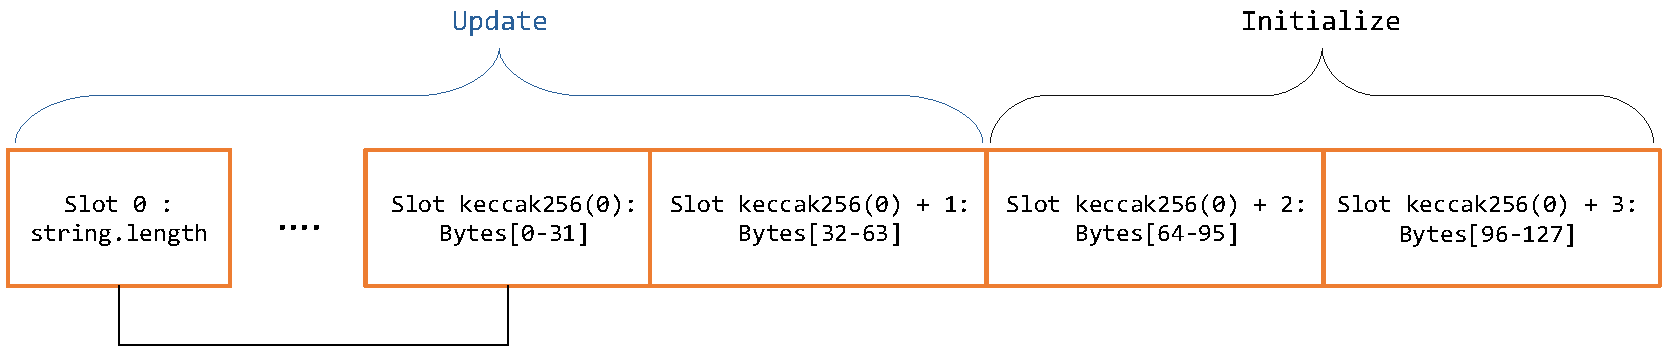
\includegraphics[width=\textwidth]{figs/Storage1.pdf}}
        \caption{}
        \label{fig:arrays_1}
    \end{subfigure}
    \begin{subfigure}{\linewidth}
        \centerline{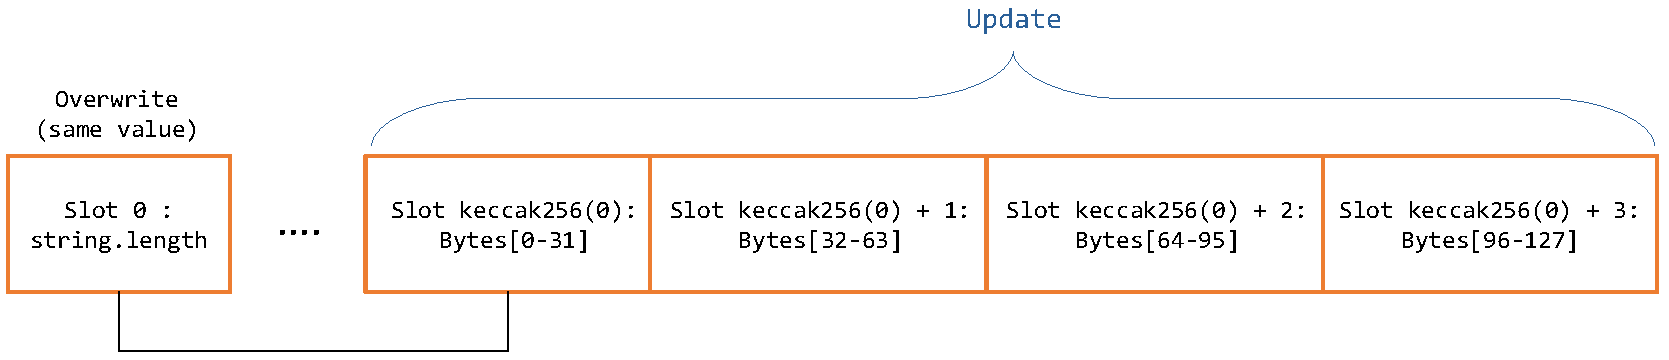
\includegraphics[width=\textwidth]{figs/Storage2.pdf}}
        \caption{}
        \label{fig:arrays_2}
    \end{subfigure}
    \caption{Slots that must updated or initialized when overwriting a string with (a) a longer (b) a new one of the same size.}
\end{figure}

In order to perform this experiment, we designed a simple SC with the following elements: a public string variable to store our data, a function to modify this string and another one to reset it. In total, we tested three of the most common scenarios.

% TODO: maybe with instead of to?
\begin{itemize}[topsep=0pt, itemsep=0pt]
  \item Storing data after resetting the variable (clean storage).
  \item Updating the variable to a longer string (double the size), Fig.~\ref{fig:arrays_1}.
  \item Updating the variable to a new string (same size), Fig.~\ref{fig:arrays_2}.
\end{itemize}

The baseline of 21000 gas for every transaction and the gas paid for its payload are equal in all three cases. So, the number of slots that must be overwritten or initialized during each test case mostly accounts for the difference in the respective costs depicted in Fig.~\ref{fig:store1} and Fig.~\ref{fig:store2}, which was included to present the costs for small data. For data less than 32 bytes, as discussed in subsection~\ref{sec:storage}, one slot is adequate. Otherwise, \(\ceil*{x/32}\) slots for storing the data and one for storing the string's size \(x\), are required. In the case of clean storage, all slots must be initialized, costing \(20000*num\_slots\) gas. When updating a string with a new one of the same size, 5000 gas is deducted for each of the \(\ceil*{x/32}\) slots. Note that the slot holding the string’s length is not updated, as the string’s size does not change. In fact it is overwritten with the same value, which is termed as a \emph{``no-op''} and is charged equally to an SLOAD operation. The second case is a combination of the others and so is the cost calculation method. Some slots must be initialized, and others need to be updated, costing 20000 and 5000 each.

\begin{figure}[htbp]
\centerline{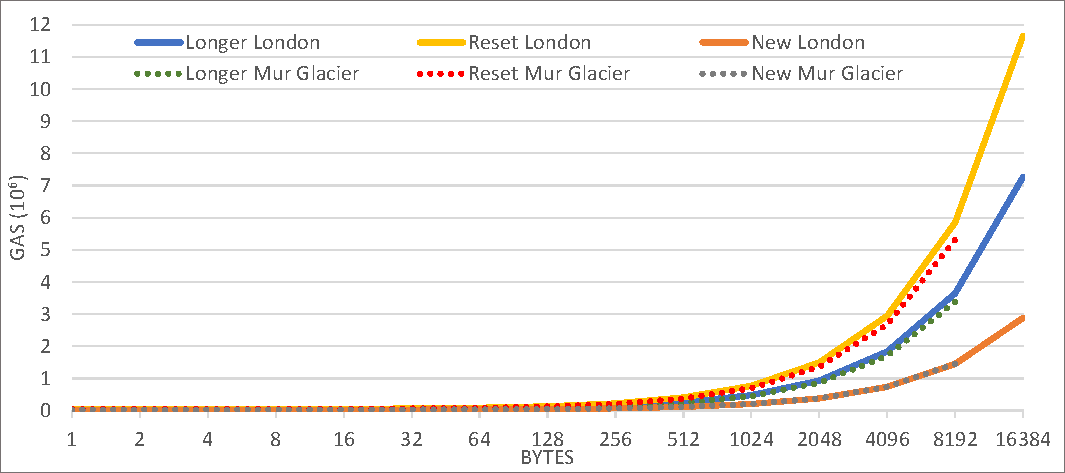
\includegraphics[width=9cm]{figs/store1.pdf}}
\caption{SC storage cost diagram.}
\label{fig:store1}
\end{figure}

\begin{figure}[htbp]
\centerline{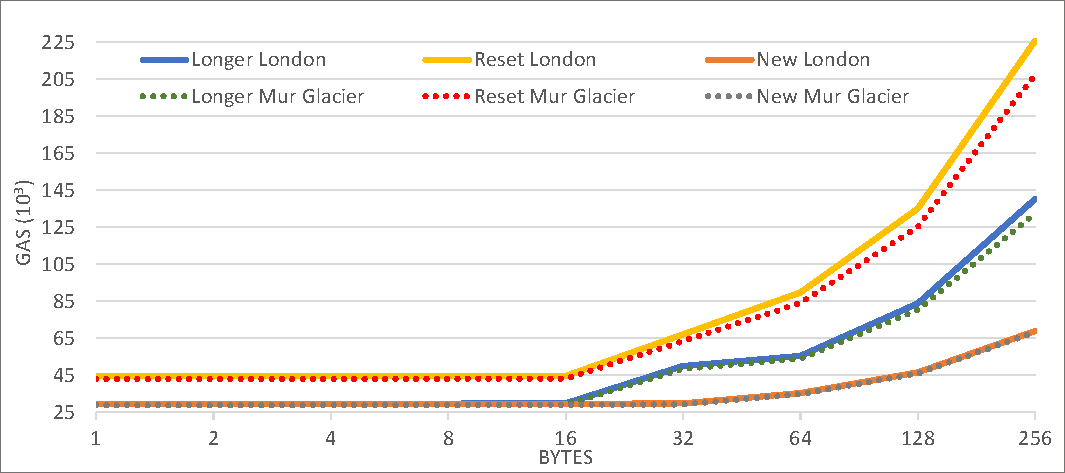
\includegraphics[width=9cm]{figs/store2.pdf}}
\caption{Zoomed in view of the diagram in Fig.~\ref{fig:store1}.}
\label{fig:store2}
\end{figure}

Up to this point, we discussed gas consumption based on the EIPs introduced prior to (including) Muir Glacier. EIP-2929, included in Berlin fork, reforms SLOAD and SSTORE gas metering.

% TODO: cite EIP-1559
Considering the altered cost model outlined in paragraph \ref{par:eip_2929_cold_warm}, we re-executed all test cases to examine Ethereum’s actual behavior after the Berlin hard fork. In order to be up-to-date, we also repeated our study when the London hard fork was implemented. Gas consumption related to the SSTORE and SLOAD operations was not altered by any of the included EIPs. However, EIP-1559 specifies a transaction pricing mechanism that temporarily raises the block’s gas limit when congestion occurs. This enabled us to store up to 16KBs in contrast to the 12KBs that we managed to store in previous experiments. In Fig.~\ref{fig:store1} we present our most recent results, since they reflect the impact that both hard forks induced.

Overall, all transactions after EIP-2929 had a higher cost, especially those regarding our first test case, in which, every slot had to be initialized imposing an overhead of 2100 gas. Regarding the third test case, all transactions executed after the fork proved to cost 600 more. By debugging those, we discovered that this difference is caused by the SLOAD gas metering modification. Basically, when updating a string, the slot that holds the string’s length is accessed twice; once to determine the string’s length (SLOAD) and a second time to update it to the new length (SSTORE). The SLOAD operation is considered a COLD\_SLOAD and costs 2100 gas. The SSTORE on the currently \emph{``warm''} slot is considered a \emph{``no-op''} since the length of the string remains the same and costs 100 gas. Before EIP-2929 took effect, these operations were charged 800 each.

\begin{figure}[htbp]
\centerline{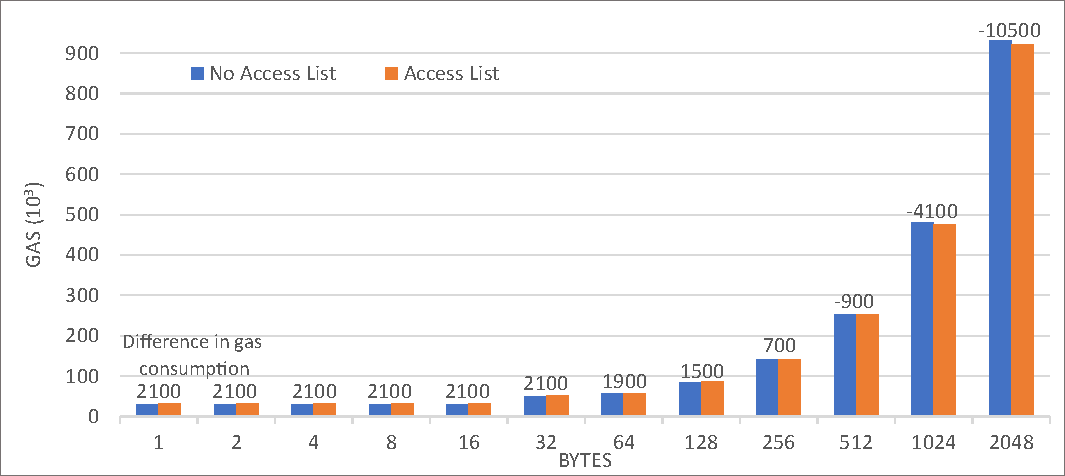
\includegraphics[width=9cm]{figs/access_list.pdf}}
\caption{SC storage cost diagram (optional AL).}
\label{fig:access_list}
\end{figure}

Besides EIP-2929, EIP-2930 was also included in the Berlin hard fork. As a result, users can now specify a list of addresses and storage keys that the transaction plans to access, which are \emph{``warmed up''} and consequently subsequent accesses come at a discounted price (see paragraph \ref{par:eip_2930_access_list}).

Based on Table~\ref{table:access_list} one would assume that declaring an AL is a better option, at all times, as 100 gas would be saved for every account/storage access and 200 gas for every SSTORE operation. However, that is not the case. If storage keys of the targeted contract are specified in an AL, the targeted contract account must be included as well, imposing an overhead of 2400 gas.
% TODO: add https://eips.ethereum.org/EIPS/eip-3521

\begin{figure}[htbp]
\centerline{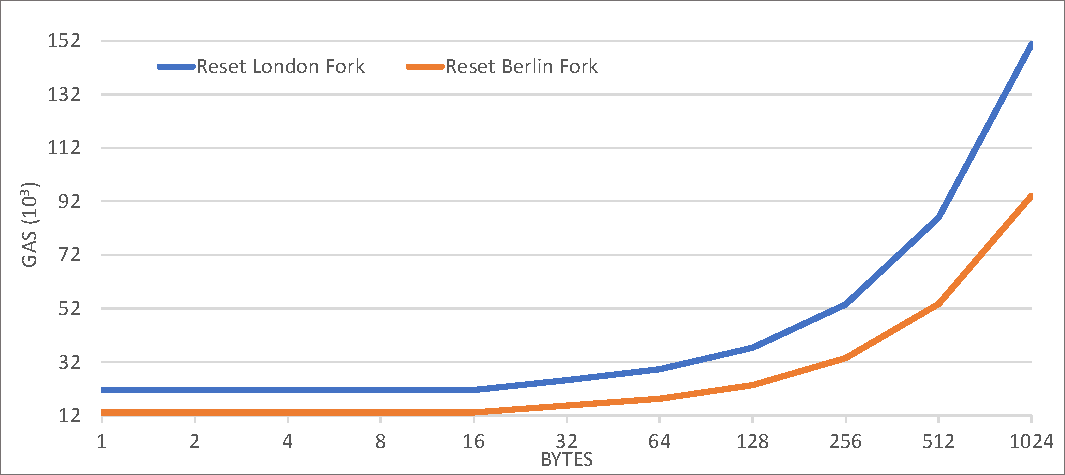
\includegraphics[width=9cm]{figs/reset.pdf}}
\caption{Cost of clearing SC storage.}
\label{fig:reset}
\end{figure}

The behavior described above is depicted in Fig.~\ref{fig:access_list}. When the string’s size is under 352 bytes, using an AL is more expensive due to the gas paid for including the contract’s address. On the contrary, storing a string longer than 352 bytes is more cost-efficient if an AL is declared. In brief, the 2400 overhead is countered by the 12 or more SSTORE operations that access each of the storage slots that contain the string's data and the SLOAD operation required to determine the string's length, which are charged at a discounted rate, i.e., 200 and 100 less gas respectively.

% TODO: if one uses access list they should refrain
As a general guide, one should opt in for the use of ALs, but refrain from specifying storage slots of the targeted contract account. Yet, if the main contract interacts with other contracts, which then access their storage, specifying their addresses (but not tx.to) and storage keys in an AL is less expensive than not using an AL.

Handling the data of a DApp involves data storage, retrieval and deletion. In Ethereum, SC storage is considered a valuable resource and therefore a gas refund is given when data is erased.

In Fig.~\ref{fig:reset}, we present the overall cost associated with clearing the slots occupied by a string’s data. Considering that clearing a slot entails updating its value from non-zero to zero, the actual execution cost is comparable to that of updating a string to a new one (see Fig.~\ref{fig:arrays_2}), except that in this case the string's length is also updated; 5000 gas is charged for every SSTORE operation on the slots that the string occupies. Though, the refund granted for these operations contributes to a lower overall transaction cost.

London hard fork introduced EIP-3529  \citep{buterin_eip_3529} which modified the refund mechanism (see paragraph \ref{par:eip_3529_refund}). Prior to this, emptying a slot was rewarded with 15000 gas and the total refund was capped at 50\% of the transaction’s gas used. In the London fork implementation both the reward and the refund were reduced to 4800 gas and 20\%, respectively. Fig.~\ref{fig:reset} demonstrates the impact that this modification has on the cost related to deleting a string. All transactions incurred an increase of approximately 38\% in gas usage.

\subsection{Event-logs}\label{subsection:evaluation_logs}

Prior to any further analysis, \hl{we ought to mention that in preliminary experiments}, counters were used as identifiers (ids) for the events, as illustrated in Table~\ref{table:event}. However, the use of counters entails the execution of an SLOAD operation, which gets their values in order to pass them as parameters to the events and also an SLOAD and SSTORE operation for incrementing them, imposing an overhead of 6600 gas in every transaction. Considering this, in our recent experiments, we decided to pass the ids as arguments. Hence, the results presented in this work are rather indicative of the effect that emitting an event has on gas consumption, as the need for extra contract logic was eliminated.

As we can observe in Fig.~\ref{fig:logs} the resulting costs from calling each event, exhibit relatively small divergence. Through  \citep{wood_2014} we know that each topic costs 375 gas. Respectively, there is a charge of 8 gas for each byte of data recorded in the data field of the logs. Thereby, the number of topics generated by the event call in each of the cases we examined, as well as the amount of data recorded in the log data field, are key factors in the cost variance between them. These are determined by the way the events are declared, as shown in Table~\ref{table:event}. If the id is indexed it is placed in the topics array along with the event’s signature hash, otherwise it is ABI encoded into the data field of the log. Additionally, since the input data are identical in all the events and the contract's code is immutable by default, the constant gap maintained by the four graphs is justified.

\begin{table*}[]
\caption{Structure of events and logs included in the experiments}
\centering
\label{table:event}
\resizebox{15cm}{!}{%
\begin{tabular}{@{}ccccc@{}}
\toprule
 & \textbf{Indexed} & \textbf{Non-Indexed} & \textbf{Anonymous Indexed} & \textbf{Anonymous} \\ \midrule
\textbf{Declaration} & \begin{tabular}[c]{@{}c@{}}event\_name(uint indexed id, \\ string data)\end{tabular} & \begin{tabular}[c]{@{}c@{}}event\_name(uint id, \\ string data)\end{tabular} & \begin{tabular}[c]{@{}c@{}}event\_name(uint indexed id, \\ string data) anonymous\end{tabular} & \begin{tabular}[c]{@{}c@{}}event\_name(uint id, \\ string data) anonymous\end{tabular} \\
\textbf{Topic{[}0{]}} & keccak(event\_signature) & keccak(event\_signature) & - & -\\
\textbf{Topic{[}1{]}} & abi\_encode(id) & - & abi\_encode(id) & - \\
\textbf{Log Data} & abi\_encode(data) & abi\_encode(id, data) & abi\_encode(data) & abi\_encode(id, data) \\ \bottomrule
\end{tabular}%
}
\end{table*}

It should be noted that because log data is ABI encoded, even a uint8 occupies 32B and is charged \( 8*32 = 256 \) gas. For this reason, converting a non-indexed parameter to an indexed does not impose much of an overhead. In fact, it is negligible since the opcodes that are executed to determine the function to be called, might result in the indexed event being less expensive. That is the case for the anonymous events, as indicated in Fig.~\ref{fig:logs}.

Finally, even though anonymous events are the least expensive option, they should be used frugally. The fact that they don’t register their signature as a topic, prohibits them from being uniquely referenced, perplexing their retrieval. Including indexed parameters to such events can assist with that.

% Finally, it is apparent that the use of SC storage incurs costs that are orders of magnitude larger than the currently discussed alternative.

\begin{figure}[htbp]
\centerline{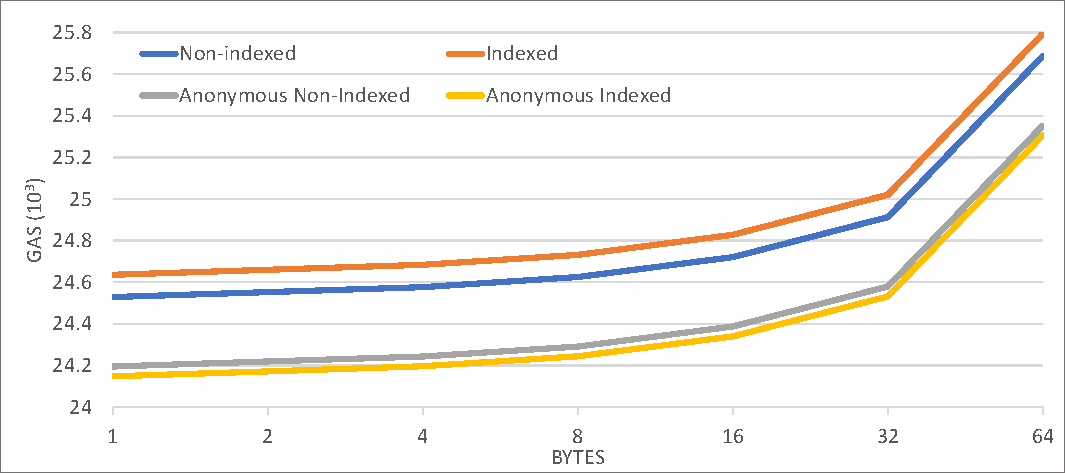
\includegraphics[width=9cm]{figs/logs_1.pdf}}
\caption{Event-logs storage cost diagram.}
\label{fig:logs}
\end{figure}

\subsection{Transaction Payload}\label{subsection:evaluation_payload}
The first step of this experiment was to encode the data in hex format. Then, we included the resulting hex byte array in the data field of a transaction object, signed it and sent it. Note that no ether was transferred during any of the transactions. We tried two different ways of implementing this method:

\begin{itemize}[topsep=0pt, itemsep=0pt]
  \item Sending the transaction between EOAs
  \item Sending the transaction from an EOA to a CA
\end{itemize}

As expected, the measurements confirm that the use of transactions as a data store is the most cost-efficient solution of all when data is sent between EOAs. As a matter of fact, this can be considered the minimum cost for storing data in Ethereum. That is, because the fee paid for a transaction’s payload is essentially included in every available option, e.g., for executing a transaction with some data as input, these data must first be sent as payload to the contract.

For the second case we tested, a fallback function in the targeted SC is required, otherwise the transactions will fail. In short, fallback is a special function that gets executed if none of the function selectors match the first four bytes of the transaction payload, or if the latter is empty and no Receive Ether function is defined. Additionally, it cannot have parameters nor return anything. The body of the fallback could either be empty or include function logic. In any case, if arbitrary hex-encoded data is included in the payload of a transaction that is targeted to a SC, the fallback will be executed (no function selector will be matched) and the data will be permanently saved in the blockchain, as part of the transaction. Implementing an empty fallback entails that the transaction hash must be saved externally. On the contrary, emitting an event inside the fallback allows the user to obtain the transaction hash from the resulting logs and retrieve the data from the recorded transaction.

\begin{figure}[htbp]
\centerline{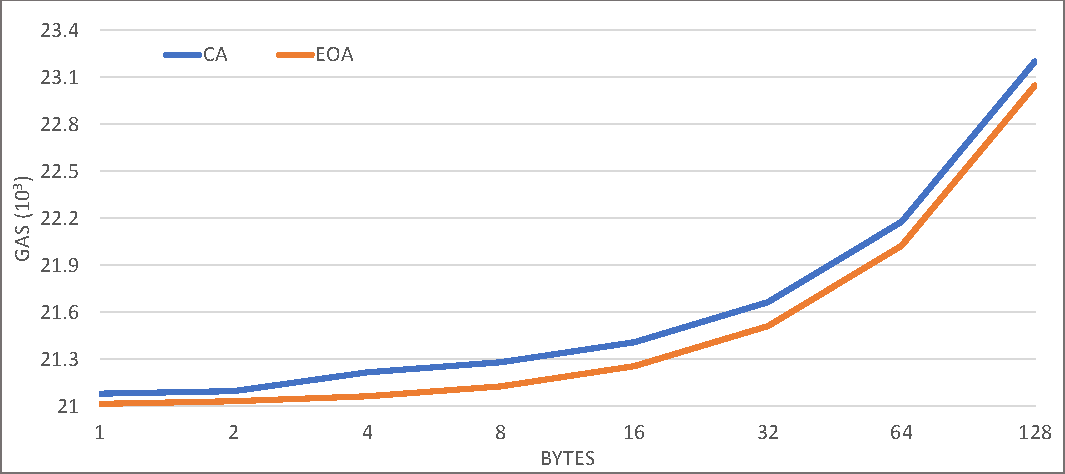
\includegraphics[width=9cm]{figs/tx.pdf}}
\caption{Transaction payload storage cost diagram.}
\label{fig:tx}
\end{figure}

Based on Fig.~\ref{fig:tx}, we are able to compare the cost of saving data in a transaction payload that is sent to an EOA or a CA, respectively. Regarding the latter scenario, the SC implements an empty fallback function. The difference between the amount of gas spent in each test case stems from the fact that in the second one some contract code needs to be executed. By inspecting the bytecode of the corresponding contract, we managed to further analyze this difference. After verifying that no ether was sent with the transaction, a series of opcodes is executed to check if the payload is less than four bytes. If that is true, EVM jumps to fallback’s execution. The accumulated cost resulting from the EVM execution, up to that point, is 65 gas greater than that of test Case 1. If the aforementioned condition is false, the first four bytes of the payload are loaded and processed, costing 12 gas, and they are compared against every function selector of our contract’s three functions. Eventually, no match is found and the execution jumps to the fallback function, which costs 10 gas. The code blocks in which the comparisons are conducted consist of the opcodes \textsc{\{dup1, push4, eq, push2, *jumpi\}}, which altogether cost 22 gas. Taking into account that no match will be found, all comparisons are executed, costing 66. In total, the cost for storing \(data\geqslant 4\) bytes in a transaction by exploiting the fallback function, is 153 gas greater than the other test case.


By inspecting the execution of the contract at bytecode level we managed to verify what to our knowledge was first reported, but not explained, in \citep{chen_2018}. Simply put, function selectors, which are comprised of the first four bytes of the Keccak-256 hash of the function's signature and therefore depend on function names and parameter types, are compared to the first four bytes of a transaction’s payload in hex-ascending order. Hence, frequently used functions should be named in an appropriate manner to avoid numerous comparisons, i.e., save gas. Moreover, we believe it is necessary to point out that for a contract with a large number of functions, Solidity optimizes the comparison flow by performing a pre-comparison to check whether the given function selector is or is not above a certain threshold.

As already mentioned, an event could be emitted inside the fallback function to avoid saving the transaction hash off-chain. Similarly to the experiments in~\ref{par:event_exp}, the event should include an id parameter so that the data can be identified upon retrieval. This was achieved in two ways: i) increasing a counter in every call ii) reserving some bytes of the transaction data (e.g., the first 32bytes) to hold the id. The latter is generic since values other than integers can be used, but requires additional logic, both on-chain and off-chain, to separate or concatenate the data and the id. In addition, eschewing the use of a counter significantly reduces the gas consumption, as depicted in Fig.~\ref{fig:fallback}. In fact, since the cost of the log operation is identical in both cases, the difference in the cost depends solely on the need of updating the counter, which involves two SLOAD and one SSTORE operations.

\begin{figure}[htbp]
\centerline{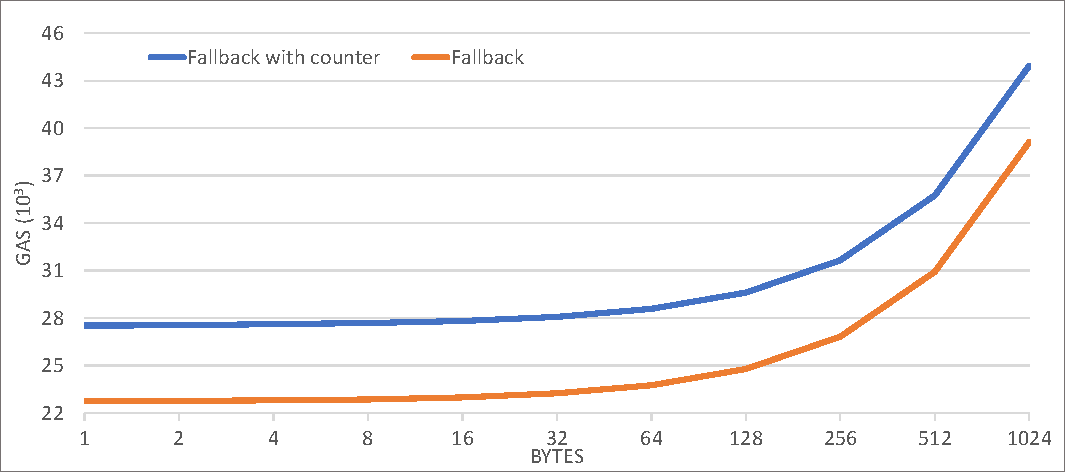
\includegraphics[width=9cm]{figs/fallback.pdf}}
\caption{Cost of emitting an event inside the fallback function.}
\label{fig:fallback}
\end{figure}

\subsection{Unused Function Parameters}\label{subsection:evaluation_unused}
This experiment was performed to examine the cost of storing data in a transaction’s payload while exploiting Solidity’s built-in ABI interface.
Such a scheme overcomes the restriction imposed by the previous method as it facilitates the management of all the data types that Solidity supports, without the need of additional client logic. 

% we used a function with a single parameter that was no further processed.
% \hl{We also decided to improve the functionality of this method by emitting an event, with just one indexed parameter, inside the function in order to track the hash of the transaction at a later point}.
In order to examine this approach, we declared a function with two parameters; one to hold the data and another one to hold an identifier. The former was no further processed, while the latter was passed to an event. Emitting an event inside the function enabled us to obtain the transaction hash from the resulting logs and retrieve the ABI encoded data from the recorded transaction. In contrast to the utilization of a fallback function, which cannot accept any arguments, the id of the event is passed as a function argument eliminating the need for additional contract logic.

To evaluate the recorded costs, we used the case of indexed events as a reference point. It is obvious from Fig.~\ref{fig:unused} that as input data grow in size, the current approach gets even cheaper than the other. The fact that in this case, no data are recorded in the data part of the produced log, accounts for the difference.

\begin{figure}[htbp]
\centerline{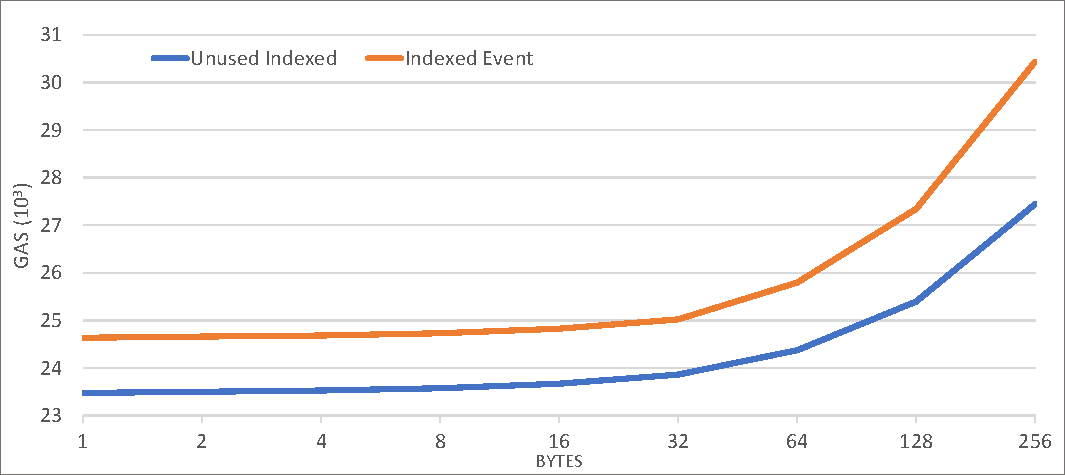
\includegraphics[width=9cm]{figs/unused.pdf}}
\caption{Unused function parameter and event-logs storage cost diagram.}
\label{fig:unused}
\end{figure}

As we already mentioned, the fact that non-indexed parameters are ABI encoded into the log data leads to long log arrays. So, in a scenario in which more unused parameters are utilized, the current approach is even less expensive. To confirm this, we conducted a complementary experiment, locally in Ganache. A contract with two functions carrying seven parameters each was deployed. Function 1 emitted an event with all parameters as input, whereas Function 2 emitted an event with just the first parameter. After executing both functions with the same arguments, we concluded that the utilization of unused function parameters can be quite effective, as Function 2 cost nearly 7000 less gas.

At this point, we would like to discuss some possible drawbacks regarding this alternative storage method. First, by testing we discovered that Solidity imposes a restriction on the number of parameters a function can bear (around sixteen). If this threshold is exceeded, a \emph{``stack too deep''} error is thrown. Additionally, defining a function with unused function parameters causes a warning at compilation. Thus, it might be disallowed in future Solidity versions.

\section{Data Retrieval in Ethereum}\label{sec:evaluation_ethereum_retrieval}
In this subsection, based on our experimental measurements, we present an overall comparison of the time needed to retrieve data from the Ethereum blockchain. Each measurement refers to the retrieval time of the data that were stored during the previous experiments. We noticed that the results were quite similar for the different data sizes (1B – 16KB), so, in Table~\ref{tab:retrieve} we recorded the average of these results. Also, we should mention that retrieving data stored in unused function parameters is a two-step process: the respective logs must be retrieved to acquire the transaction hash and then the transaction itself must be retrieved to acquire the targeted data. Likewise, using events without indexed parameters implies that additional logic should be implemented to find the desired data among the returned events. In any case, these delays were found to be insignificant compared to the time needed to retrieve the respective events. Thus, all measurements presented in Table~\ref{tab:retrieve} include any necessary additional step.

Considering the measurements presented in Table~\ref{tab:retrieve}, it is obvious that both retrieving data from contract’s storage or retrieving a transaction and extracting its data, require substantially less time than that of the other test cases. That is because these particular retrieval processes are ultimately single database queries that target either the Storage Trie or a Transaction Trie. 

\begin{table}[]
\caption{Retrieval latency in Ethereum (ms)}
\label{tab:retrieve}
\centering
\resizebox{12cm}{!}{%
\begin{tabular}{@{}ccc@{}}
\toprule
 & \multicolumn{2}{c}{\textbf{Retrieval Latency}} \\ \midrule
\textbf{Storage}&\multicolumn{2}{c}{0.89}\\
\textbf{Transaction}&\multicolumn{2}{c}{1.79}\\
\midrule
\textbf{} & \textbf{fromBlock: 0} & \textbf{\begin{tabular}[c]{@{}c@{}}fromBlock: con\_creation\end{tabular}} \\ \midrule
\textbf{Non Indexed Event}&331.33&39.16\\
\textbf{Indexed Event}&276.62&33.04\\
\textbf{Anonymous Event}&1569.76&67.55\\
\textbf{Anonymous Indexed Event}&420.60&36.85\\
\textbf{Unused Inexed Event}&276.44&30.19\\
\textbf{Unused Non Indexed Event}&337.01&34.59\\
\bottomrule
\end{tabular}%
}
\end{table}

On the other hand, the process of retrieving events involves the utilization of BFs and therefore is more complex and leads to higher latency. Though, through an appropriate interface, a developer can specify the block from which the client should start searching for the requested event(s). This can greatly reduce the number of database queries, as less BFs need to be inspected, resulting in faster retrieval. Indeed, we confirmed that searching from the beginning of the blockchain as opposed to specifying a more recent starting point requires significantly more time. In our experiments, as a starting block, we set the ones that our contracts were deployed in since no events could have been emitted before that point. Besides that, we observe that the use of indexed parameters in an event can further improve the retrieval performance.

As mentioned in subsection ~\ref{par:bloom}, three bits of the BF are set by the contract’s address and three for every topic. Anonymous events don’t register their signature hash as a topic. Thereby, filtering an anonymous event with no indexed parameters is accomplished by verifying that the three bits that correspond to the contract’s address are set in the BF. However, every event of the same contract would have set these bits as well. In a similar manner, the bits set by the anonymous indexed event we declared, are also set by every other indexed event; given the same uint256 as input for the indexed parameter, the bits they set coincide. The behavior we describe is demonstrated in Fig.~\ref{fig:bloom_combined}. In brief, anonymous events result in a higher false positive rate thus hindering the retrieval process.


\begin{figure}
    \begin{subfigure}{\linewidth}
        \centerline{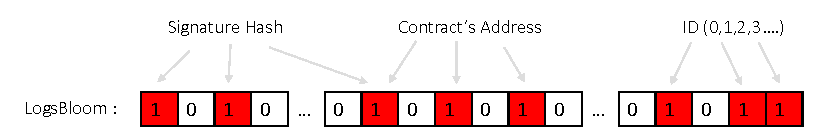
\includegraphics[width=9cm]{figs/bloom_indexed.pdf}}
        \caption{}
        \label{fig:bloom_indexed}
    \end{subfigure}
    \begin{subfigure}{\linewidth}
        \centerline{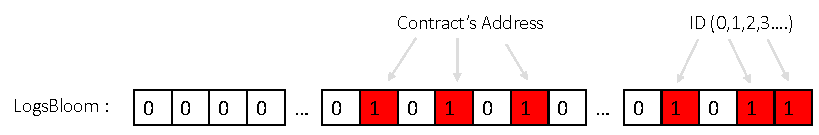
\includegraphics[width=9cm]{figs/bloom_anonymous.pdf}}
        \caption{}
        \label{fig:bloom_anonymous}
    \end{subfigure}
    \caption{Example of the bloom bits set by (a) indexed (b) anonymous indexed events.}
    \label{fig:bloom_combined}
\end{figure}

It is noteworthy that Geth uses LevelDB to manage the blockchain's data. Driven by the fact that most operating systems utilize free RAM memory for caching, we decided to assess how the system’s cache may influence the retrieval performance. In short, recently accessed LevelDB files are cached by the OS and therefore subsequent requests are served faster. So, we repeated our experiments but dropped the page cache between each run, as it is proposed in  \citep{perez_2020}, and gathered the measurements in Table~\ref{tab:retrieve_clear}. This dramatically delayed the retrieval of data from logs when the starting block was set to zero (i.e., beginning of the chain). Basically, when filtering from block zero, a lot of LevelDB files are accessed to find a specific log. The fact that these files are loaded from disk when they are not available in the system’s cache, justifies this delay. On the other hand, since the required disk accesses are greatly reduced when the search is conducted with a more recent starting point, the retrieval latency is not affected to the same extent.

\begin{table}[htbp]
\caption{Retrieval latency in Ethereum with clear cache (ms)}
\label{tab:retrieve_clear}
\centering
\resizebox{12cm}{!}{%
\begin{tabular}{@{}ccc@{}}
\toprule
 & \multicolumn{2}{c}{\textbf{Retrieval Latency}} \\ \midrule
\textbf{Storage}&\multicolumn{2}{c}{1.95}\\
\textbf{Transaction}&\multicolumn{2}{c}{3.98}\\
\midrule
\textbf{} & \textbf{fromBlock: 0} & \textbf{\begin{tabular}[c]{@{}c@{}}fromBlock: con\_creation\end{tabular}} \\ \midrule
\textbf{Non Indexed Event}&1156.90&44.78\\
\textbf{Indexed Event}&1128.71&33.54\\
\textbf{Anonymous Event}&4034.35&78.19\\
\textbf{Anonymous Indexed Event}&1289.72&38.84\\
\textbf{Unused Inexed Event}&1136.50&31.93\\
\textbf{Unused Non Indexed Event}&1154.05&39.29\\
\bottomrule
\end{tabular}%
}
\end{table}

\begin{table*}[!h]
 \centering
\caption{Overall comparison of Ethereum's data stores.}
\label{table:overall}
\begin{tabular}{@{}p{0.1\linewidth}p{0.09\linewidth} p{0.09\linewidth}p{0.09\linewidth}p{0.55\linewidth}@{}}
\toprule
 &  & \textbf{Storage Cost} & \textbf{Retrieval Latency} & \textbf{Comments} \\* \midrule
\textbf{Storage} & & Very High  & Very Low & \multirow{3}{10cm}{Viable option only when storing small data. Should host all the data that is essential for the SC's proper operation, since data stored using any of the alternative methods is not accessible within the SC. }\\\\\\* \midrule
\multirow{4}{*}{\textbf{Event-logs}} & \textbf{Non-Indexed}& Low&Moderate &\multirow{4}{10cm}{Suitable for archiving data at a low cost. Filtering specific logs is time consuming but limiting the filtering block-range and exploiting indexed parameters can accelerate the process. Thus, events should be declared according to the DApps' needs, so that %when retrieval performance matters,%
high latency is avoided.} \\
 & \textbf{Indexed} &Low&Moderate   \\
 & \textbf{Anonymous} & Low & Very High  \\
 & \textbf{Anonymous Indexed} &Low & High   \\* \midrule
\textbf{Transaction Payload} & \textbf{CA} &Very Low - Moderate& Very Low - Very High & \multirow{3}{10cm}{Least expensive method if the target is an EOA. The transaction hashes must be saved off-chain. In case of transactions to CAs, the cost and the retrieval performance are effected by the manner the SC's fallback is implemented.} \\

% The most cost-efficient method when transactions are targeted to EOAs. Transaction hashes must be saved off-chain. For transactions to CAs cost and retrieval performance are effected by the type of the event emitted in the fallback

\textbf{} & \textbf{EOA} &Very Low& Very Low \\\\* \midrule
\textbf{Unused functions parameters} & & Very Low  & Very Low - Very High  &\multirow{4}{10cm}{A useful variant of the previous method. Data is essentially stored in the transaction payload but the ABI specification is exploited, facilitating the management of all supported data types. Events can be used for tracking the transaction hashes at the expense of retrieval performance.}\\\\\\* \bottomrule
\end{tabular}%
% }
\end{table*}

To sum up, retrieving logs is time-consuming and imposes an overhead in most of the methods we proposed. However, one can make this compromise considering the cost reduction that these alternatives bring. Apart from that, if managing an external database for storing the transaction hashes is not discouraging, data could be stored in a transaction’s payload or even in unused function parameters, without emitting an event, which imposes an extra cost. By doing so, the cost as well as the retrieval time are reduced substantially.

\section{IPFS \& SWARM}\label{sec:evaluation_dfs}
The aim of this experiment was to examine the use of IPFS and Swarm alongside Ethereum. We stored data blocks of size 4KB–16MB in these platforms and recorded the resulting identifiers in Ethereum using both SC storage and logs. The cost related to storing these identifiers in Ethereum was examined as well. 

Details about remote experiments...
\subsection{Storing data identifiers in Ethereum}\label{subsection:evaluation_identifiers}
In general, the cost of recording content identifiers in Ethereum is consistent due to the constant length of the identifiers. However, in IPFS, using a CID v1 instead of CID v0, will result in higher gas consumption as it requires more storage space. CID v1 format \citep{multiformat}, which will be the default in the near future, consists of four parts

% \[\textsc <cidv1> ::= <multibase><multicodec-version><multicodec-content-type><multihash>\]

\begin{flushleft}
\centering
$\textsc <cidv1> ::= <multibase><multicodec-version><multicodec-content-type><multihash>$
\end{flushleft}

while CID v0 contains only the \(\scriptstyle <multihash>\), which is always a SHA-256 multihash \citep{multiformat}, i.e., a 34-byte hex array with the leading bytes [0x12, 0x20], used to denote the hash function and the hash digest’s size, followed by the hash digest. The rest are implicitly assumed to be (base58btc - cidv0 - dag-pb).

Below, we briefly describe three different approaches we studied and present the related cost concerning the use of SC storage and logs as a data store for the identifiers:

\begin{itemize}[topsep=0pt, itemsep=0pt]
\item{Save the CID in its original form (string).}
\item{Save just the hash digest of the multihash in a bytes32 data type.} 
\item{Save all parts of the CID separately, either in a struct or in an event with five parameters.}
\end{itemize}

In the last scenario, the struct is declared in an appropriate manner so that the version, the content-type and the multihashe’s function code and digest size are grouped together in a single slot. The hash digest occupies a separate slot. However, since a CID encoded in any multibase points to the same content, storing it is optional.

Based on Table~\ref{tab:hash_cost}, we conclude that storing only the hash digest of the CID, is the least expensive option. That is because in storage it takes up just one storage slot and also results in the shortest log byte array. However, this approach has a downside. A hash digest cannot be converted back to a CID v1 without the hash function code, multicodec, etc. Hence, this information must be stored off-chain or the DApp would be able to handle only CIDs v0.

\begin{table}[htbp]
\centering
\caption{Cost of storing data identifiers (gas)}
\label{tab:hash_cost}
\resizebox{12cm}{!}{%
\begin{tabular}{@{}lcccc@{}}
\toprule
 & \multicolumn{2}{c}{\textbf{IPFS}} & \multicolumn{2}{c}{\textbf{Swarm}} \\* \midrule
 & \textbf{CID0} & \textbf{CID1} & \textbf{Unencrypted} & \textbf{Encrypted} \\* \midrule
\textbf{Original form (logs)}&24825&24981&23262&25086\\
\textbf{Original form (storage)}&89542&89741&44141&89757\\
\textbf{Broken down CID (logs)}&25883&25931&-&-\\
% Remix: CID0 26575 CID1 26635
\textbf{Broken down CID (storage)}&48682&68630&-&-\\
% Remix: CID0 49266 CID1 69226
\textbf{Hash digest (logs)}&23240&23240&-&-\\
\textbf{Hash digest (storage)}&44207&44207&-&-\\* \bottomrule
\end{tabular}%
}
\end{table}

The use of logs as a data store for the identifiers leads to higher retrieval latency but, be that as it may, it’s definitely a more affordable option. Actually, one would prefer to log the CID in its original form, rather than declaring an event with five parameters to hold the CID’s individual parts. The latter is more expensive since the parameters need to be ABI encoded, taking up more bytes than the complete CID. On top of that, the CID has to be reassembled to its original form.

In all the test cases we examined, the CIDs v1 were generated using the SHA-256 hash function (default option). Hash functions that produce a shorter or same-sized hash digest would result in similar gas consumption whereas hash functions like SHA-512 would increase the cost, since additional storage slots or longer log arrays would be necessary to store them.

As discussed in Section~\ref{subsec:distributed}, when it comes to Swarm, the identifiers’ representation is fairly simple. For unencrypted content 32 bytes suffice, otherwise 64 bytes are required. Thus, gas consumption in Swarm’s case is straightforward. A developer, based on the above table can choose the appropriate method.
\subsection{Local Upload \& Retrieval Performance}\label{subsection:evaluation_local}
The measurements presented in Fig.~\ref{fig: ipfs_swarm_upload}, indicate that uploading data up to 256KB in Swarm is quite fast. Above this threshold, performance deteriorates substantially. We must consider that data are split into chunks which are hashed and organized in a Binary Merkle Tree. Obviously, the number of calculations included in this process is proportional to the size of the data and definitely affects the upload-time.

IPFS behaves similarly, except that the size of the data has smaller impact on its performance. This mostly stems from the fact that chunk’s default size (256KB) in IPFS is 64 times the size of a Swarm chunk (4KB), rendering the process of splitting the data and organizing the chunks in a Merkle-Dag faster. Accordingly, the quite stable measurements for data up to 256KB are justified, as they fit in one chunk. To substantiate this claim, we uploaded data on IPFS with the chunker option set to 4KB instead of 256KB. In all tests, the upload latency increased significantly. In fact, Swarm proved to be far more efficient in this scenario. On top of that, the different algorithms and data structures used by each platform to split, store and link data, contribute to the performance gap between them.

\begin{figure}[htbp]
\centerline{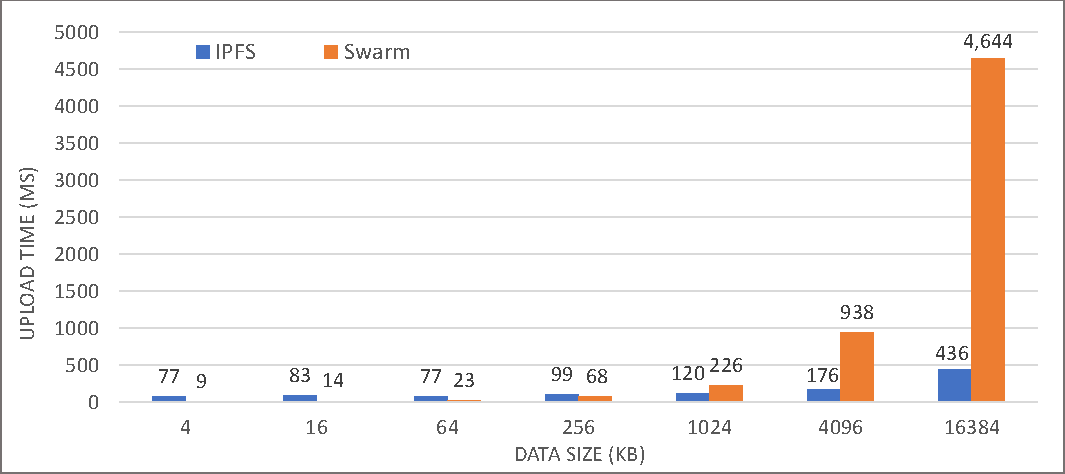
\includegraphics[width=9cm]{figs/ipfs_swarm_upload.pdf}}
\caption{IPFS-Swarm upload latency.}
\label{fig: ipfs_swarm_upload}
\end{figure}
\setlength{\belowcaptionskip}{-10pt}

As we can observe from Fig.~\ref{fig: ipfs_swarm_retrieve}, Swarm lacks in performance when it comes to retrieving data from local storage. That is due to the fact that all chunks split during the upload process must be individually fetched in order to reconstruct the original data. A large number of chunks implies a complex Merkle-Tree or Merkle-DAG. Thus, longer paths have to be resolved until each chunk is found, leading to greater retrieval time. Once again, it is clear that the chunk-size utilized within each platform’s architecture is a determining factor for their performance.

\begin{figure}[htbp]
\centerline{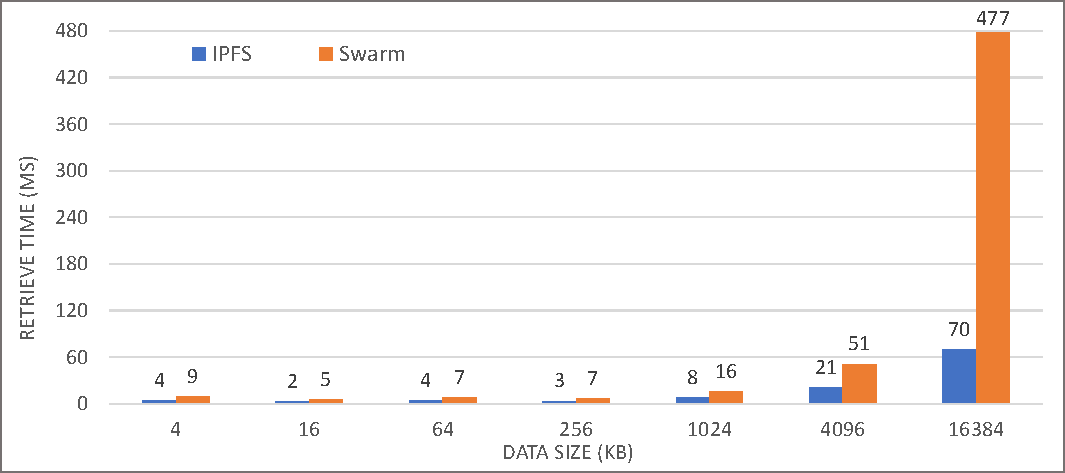
\includegraphics[width=9cm]{figs/ipfs_swarm_retrieve.pdf}}
\caption{IPFS-Swarm retrieval latency.}
\label{fig: ipfs_swarm_retrieve}
\end{figure}
\setlength{\belowcaptionskip}{-10pt}

We ought to clarify that by conducting these experiments we meant to compare the performance of IPFS and Swarm, regarding local upload and retrieval. The results are nothing but representative of how these platforms behave when exchanging data between remote nodes. Besides that, Swarm updated its networking protocol from DevP2P to LibP2P and introduced a new client, which we used during our experiments. The fact that it is in primary stage and improvements are frequently made might render our results obsolete in the near future.
\subsection{Remote Upload and Retrieval Performance}\label{subsection:evaluation_remote}

% \paragraph{IPFS}
% % Please add the following required packages to your document preamble:
% % \usepackage{booktabs}
% \begin{table}[H]
% \caption{Table for experiment disconnect}
% \begin{tabular}{@{}lcccccccc@{}}
% \toprule
% Host    & \multicolumn{7}{c}{Data Size}          & Sample Size \\ \midrule
% & 4kb  & 16kb  & 64kb  & 256kb  & 1mb  & 4mb  & 16mb              \\ \midrule
% chetemi-9.lille  & 612  & 282  & 1010  & 891  & 1679  & 2264  & 1929  & 16 \\
% dahu-32.grenoble  & 146  & 456  & 2133  & 679  & 1065  & 857  & 1158  & 16 \\
% degroot  & 1933  & 2014  & 2192  & 1622  & 1892  & 2639  & 3028  & 30 \\
% graphite-4.nancy  & 835  & 1352  & 1868  & 723  & 1305  & 1440  & 1980  & 24 \\
% paravance-51.rennes  & 1097  & 2360  & 4096  & 2835  & 1403  & 2882  & 1874  & 18 \\
% uvb-9.sophia  & 425  & 617  & 3902  & 1056  & 1228  & 779  & 1796  & 16 \\
% \bottomrule
% \end{tabular}
% \end{table}

% % Please add the following required packages to your document preamble:
% % \usepackage{booktabs}
% \begin{table}[H]
% \caption{Table for experiment do-not-cache}
% \begin{tabular}{@{}lcccccccc@{}}
% \toprule
% Host    & \multicolumn{7}{c}{Data Size}          & Sample Size \\ \midrule
% & 4kb  & 16kb  & 64kb  & 256kb  & 1mb  & 4mb  & 16mb             \\ \midrule
% chetemi-9.lille  & 1560  & 80  & 96  & 120  & 133  & 433  & 574  & 8 \\
% dahu-9.grenoble  & 1189  & 261  & 111  & 134  & 142  & 228  & 602  & 8 \\
% degroot  & 1457  & 162  & 1349  & 293  & 344  & 482  & 1374  & 13 \\
% graphite-1.nancy  & 980  & 70  & 100  & 134  & 139  & 221  & 611  & 11 \\
% paravance-8.rennes  & 2564  & 69  & 101  & 130  & 150  & 214  & 555  & 11 \\
% uvb-9.sophia  & 3788  & 1441  & 104  & 148  & 164  & 262  & 798  & 8 \\
% \bottomrule
% \end{tabular}
% \end{table}

% % Please add the following required packages to your document preamble:
% % \usepackage{booktabs}
% \begin{table}[H]
% \caption{Table for experiment do-not-cache-disconnect}
% \begin{tabular}{@{}lcccccccc@{}}
% \toprule
% Host    & \multicolumn{7}{c}{Data Size}          & Sample Size \\ \midrule
% & 4kb  & 16kb  & 64kb  & 256kb  & 1mb  & 4mb  & 16mb             \\ \midrule
% chetemi-9.lille  & 83  & 485  & 1033  & 1122  & 1164  & 2281  & 1549  & 4 \\
% dahu-32.grenoble  & 707  & 992  & 895  & 1144  & 1627  & 983  & 1713  & 7 \\
% degroot  & 1407  & 1441  & 1552  & 1605  & 1925  & 3428  & 2802  & 16 \\
% graphite-4.nancy  & 743  & 2391  & 686  & 710  & 2416  & 693  & 2042  & 8 \\
% paravance-51.rennes  & 667  & 938  & 288  & 592  & 1351  & 988  & 1194  & 7 \\
% uvb-9.sophia  & 103  & 499  & 1760  & 895  & 2538  & 1274  & 2691  & 4 \\
% \bottomrule
% \end{tabular}
% \end{table}

% % Please add the following required packages to your document preamble:
% % \usepackage{booktabs}
% \begin{table}[H]
% \caption{Table for experiment normal}
% \begin{tabular}{@{}lcccccccc@{}}
% \toprule
% Host    & \multicolumn{7}{c}{Data Size}          & Sample Size \\ \midrule
% & 4kb  & 16kb  & 64kb  & 256kb  & 1mb  & 4mb  & 16mb             \\ \midrule
% chetemi-9.lille  & 308  & 139  & 186  & 257  & 1549  & 519  & 1606  & 21 \\
% dahu-32.grenoble  & 453  & 123  & 165  & 219  & 252  & 588  & 1539  & 23 \\
% degroot  & 849  & 161  & 204  & 287  & 439  & 802  & 2260  & 25 \\
% graphite-4.nancy  & 357  & 120  & 150  & 191  & 247  & 464  & 1291  & 23 \\
% paravance-51.rennes  & 397  & 117  & 166  & 215  & 232  & 411  & 1527  & 24 \\
% uvb-9.sophia  & 432  & 145  & 175  & 248  & 325  & 672  & 2079  & 24 \\
% \bottomrule
% \end{tabular}
% \end{table}



% \paragraph{IPFS - miletus degroot nancy}
% % Please add the following required packages to your document preamble:
% % \usepackage{booktabs}
% \begin{table}[H]
% \caption{Table for experiment disconnect}
% \begin{tabular}{@{}lcccccccc@{}}
% \toprule
% Host    & \multicolumn{7}{c}{Data Size}          & Sample Size \\ \midrule
% & 4kb  & 16kb  & 64kb  & 256kb  & 1mb  & 4mb  & 16mb             \\ \midrule
% degroot  & 945  & 639  & 2375  & 771  & 1761  & 801  & 3308  & 12 \\
% graphite-3.nancy  & 1618  & 938  & 1601  & 4838  & 1653  & 2231  & 5079  & 12 \\
% miletus  & 443  & 2086  & 1064  & 3974  & 2504  & 3101  & 7313  & 12 \\
% \bottomrule
% \end{tabular}
% \end{table}

% % Please add the following required packages to your document preamble:
% % \usepackage{booktabs}
% \begin{table}[H]
% \caption{Table for experiment do-not-cache}
% \begin{tabular}{@{}lcccccccc@{}}
% \toprule
% Host    & \multicolumn{7}{c}{Data Size}          & Sample Size \\ \midrule
% & 4kb  & 16kb  & 64kb  & 256kb  & 1mb  & 4mb  & 16mb             \\ \midrule
% degroot  & 158  & 100  & 117  & 143  & 232  & 522  & 2008  & 16 \\
% graphite-3.nancy  & 244  & 152  & 164  & 195  & 288  & 678  & 1881  & 15 \\
% miletus  & 173  & 155  & 102  & 170  & 501  & 1269  & 3672  & 14 \\
% \bottomrule
% \end{tabular}
% \end{table}

% % Please add the following required packages to your document preamble:
% % \usepackage{booktabs}
% \begin{table}[H]
% \caption{Table for experiment do-not-cache-disconnect}
% \begin{tabular}{@{}lcccccccc@{}}
% \toprule
% Host    & \multicolumn{7}{c}{Data Size}          & Sample Size \\ \midrule
% & 4kb  & 16kb  & 64kb  & 256kb  & 1mb  & 4mb  & 16mb             \\ \midrule
% degroot  & 1993  & 343  & 755  & 385  & 3017  & 1207  & 2705  & 12 \\
% graphite-3.nancy  & 532  & 909  & 1141  & 1285  & 1486  & 4015  & 2876  & 7 \\
% miletus  & 302  & 1790  & 6352  & 1328  & 2343  & 3955  & 6663  & 9 \\
% \bottomrule
% \end{tabular}
% \end{table}

% % Please add the following required packages to your document preamble:
% % \usepackage{booktabs}
% \begin{table}[H]
% \caption{Table for experiment normal}
% \begin{tabular}{@{}lcccccccc@{}}
% \toprule
% Host    & \multicolumn{7}{c}{Data Size}          & Sample Size \\ \midrule
% & 4kb  & 16kb  & 64kb  & 256kb  & 1mb  & 4mb  & 16mb             \\ \midrule
% degroot  & 200  & 105  & 123  & 144  & 232  & 503  & 1810  & 16 \\
% graphite-3.nancy  & 159  & 145  & 160  & 179  & 208  & 381  & 1258  & 16 \\
% miletus  & 362  & 275  & 194  & 214  & 521  & 1738  & 6155  & 16 \\
% \bottomrule
% \end{tabular}
% \end{table}




% \paragraph{Swarm}

% % Please add the following required packages to your document preamble:
% % \usepackage{booktabs}
% \begin{table}[H]
% \caption{Table for experiment disconnect}
% \begin{tabular}{@{}lcccccccc@{}}
% \toprule
% Host    & \multicolumn{7}{c}{Data Size}          & Sample Size \\ \midrule
% & 4kb  & 16kb  & 64kb  & 256kb  & 1mb  & 4mb  & 16mb             \\ \midrule
% chetemi-9.lille  & 23  & 106  & 316  & 294  & 1038  & 2725  & 8410  & 9 \\
% dahu-9.grenoble  & 86  & 225  & 376  & 460  & 1146  & 3384  & 9339  & 9 \\
% degroot  & 148  & 347  & 425  & 620  & 2008  & 5025  & 9884  & 3 \\
% graphite-4.nancy  & 63  & 208  & 327  & 432  & 1102  & 3129  & 7469  & 9 \\
% paravance-9.rennes  & 58  & 179  & 402  & 360  & 1018  & 3341  & 8612  & 10 \\
% uvb-9.sophia  & 87  & 255  & 451  & 534  & 1377  & 3834  & 9508  & 6 \\
% \bottomrule
% \end{tabular}
% \end{table}

% % Please add the following required packages to your document preamble:
% % \usepackage{booktabs}
% \begin{table}[H]
% \caption{Table for experiment do-not-cache}
% \begin{tabular}{@{}lcccccccc@{}}
% \toprule
% Host    & \multicolumn{7}{c}{Data Size}          & Sample Size \\ \midrule
% & 4kb  & 16kb  & 64kb  & 256kb  & 1mb  & 4mb  & 16mb             \\ \midrule
% chetemi-9.lille  & 13  & 135  & 153  & 343  & 895  & 2671  & 6304  & 5 \\
% dahu-9.grenoble  & 34  & 224  & 287  & 476  & 1189  & 3512  & 11754  & 6 \\
% degroot  & 104  & 327  & 521  & 778  & 1744  & 4632  & 13793  & 9 \\
% graphite-4.nancy  & 16  & 187  & 203  & 475  & 1153  & 3050  & 7832  & 4 \\
% paravance-9.rennes  & 21  & 154  & 146  & 444  & 983  & 3155  & 7520  & 3 \\
% uvb-9.sophia  & 54  & 292  & 280  & 489  & 1136  & 3402  & 11738  & 6 \\
% \bottomrule
% \end{tabular}
% \end{table}

% % Please add the following required packages to your document preamble:
% % \usepackage{booktabs}
% \begin{table}[H]
% \caption{Table for experiment do-not-cache-disconnect}
% \begin{tabular}{@{}lcccccccc@{}}
% \toprule
% Host    & \multicolumn{7}{c}{Data Size}          & Sample Size \\ \midrule
% & 4kb  & 16kb  & 64kb  & 256kb  & 1mb  & 4mb  & 16mb             \\ \midrule
% chetemi-9.lille  & 34  & 151  & 177  & 405  & 876  & 2616  & 7975  & 5 \\
% dahu-9.grenoble  & 33  & 231  & 285  & 447  & 1073  & 3155  & 9418  & 5 \\
% degroot  & 222  & 358  & 372  & 1040  & 1698  & 5321  & 11447  & 2 \\
% graphite-4.nancy  & 32  & 234  & 326  & 382  & 920  & 2827  & 7647  & 5 \\
% paravance-9.rennes  & 37  & 215  & 316  & 439  & 1043  & 3370  & 8176  & 6 \\
% uvb-9.sophia  & 105  & 229  & 337  & 449  & 1212  & 3343  & 8950  & 6 \\
% \bottomrule
% \end{tabular}
% \end{table}

% % Please add the following required packages to your document preamble:
% % \usepackage{booktabs}
% \begin{table}[H]
% \caption{Table for experiment normal}
% \begin{tabular}{@{}lcccccccc@{}}
% \toprule
% Host    & \multicolumn{7}{c}{Data Size}          & Sample Size \\ \midrule
% & 4kb  & 16kb  & 64kb  & 256kb  & 1mb  & 4mb  & 16mb             \\ \midrule
% chetemi-9.lille  & 49  & 81  & 191  & 289  & 673  & 2086  & 9710  & 11 \\
% dahu-9.grenoble  & 43  & 171  & 220  & 440  & 864  & 2633  & 9461  & 11 \\
% degroot  & 119  & 331  & 524  & 621  & 1721  & 4418  & 12738  & 11 \\
% graphite-4.nancy  & 32  & 186  & 229  & 426  & 915  & 2838  & 8037  & 8 \\
% paravance-9.rennes  & 64  & 144  & 278  & 447  & 1017  & 2967  & 9319  & 10 \\
% uvb-9.sophia  & 58  & 175  & 195  & 453  & 895  & 2677  & 10532  & 10 \\
% \bottomrule
% \end{tabular}
% \end{table}
